\documentclass[class=report, float=false, crop=false]{standalone}

\usetheme{Warsaw}
% \usecolortheme{spruce}

%%%%% PACKAGES

\usepackage{graphicx} % figures
\usepackage{multimedia} % videos
\usepackage{url}
\usepackage{amsmath}
\usepackage{amssymb}
\everymath{\displaystyle}
\usepackage{epstopdf} % conversion from .eps to .pdf
\usepackage[utf8]{inputenc}
\usepackage[T1]{fontenc}
\usepackage{upgreek}
\usepackage{nameref}
\usepackage{url}
\usepackage{pgf, tikz}
\usepackage{float}
\usepackage[english]{babel}
\usepackage{caption}
\usepackage{subcaption}
\usepackage{fontawesome5}
\usepackage{xcolor}

\usepackage{biblatex}
\addbibresource{references/biblio.bib}

%%%%% TEMPLATE

\captionsetup{font=scriptsize,labelfont={scriptsize, color=blue}}

\AtBeginSubsection[]
{
 \begin{frame}<beamer>{}
   \tableofcontents[currentsection,currentsubsection]
 \end{frame}
}
\AtBeginSection[]
{
  \begin{frame}<beamer>{}
    \tableofcontents[currentsection]
  \end{frame}
}

\defbeamertemplate*{footline}{mytheme}%
{  \begin{beamercolorbox}[ht=2.5ex]{bordure}
\begin{beamercolorbox}[wd=0.2\paperwidth,ht=2.5ex,dp=1ex,center]{author in head/foot}%
\usebeamerfont{author in head}\insertshortauthor
\end{beamercolorbox}%
\begin{beamercolorbox}[wd=0.57\paperwidth,ht=2.5ex,dp=1ex,center]{title in head/foot}%
\usebeamerfont{title in head/foot}\insertshorttitle
\end{beamercolorbox}%
% \begin{beamercolorbox}[wd=0.4\paperwidth,ht=2.5ex,dp=1ex,center]{title in head/foot}%
% \usebeamerfont{title in head/foot}\insertdate
% \end{beamercolorbox}%
\begin{beamercolorbox}[wd=0.12\paperwidth,ht=2.5ex,dp=1ex,center]{title in head/foot}%
\usebeamerfont{title in head/foot}\insertdate
\end{beamercolorbox}%
\begin{beamercolorbox}[wd=0.11\paperwidth,ht=2.5ex,dp=1ex,center]{date in head/foot}%
\usebeamerfont{date in head/foot}\insertframenumber /\inserttotalframenumber{}\hspace{2ex}
\end{beamercolorbox}%

  \end{beamercolorbox}
}

% \defbeamertemplate*{headline}{mytheme}%
% {  \begin{beamercolorbox}[ht=2.5ex]{bordure}
% \begin{beamercolorbox}[wd=\paperwidth,ht=2.5ex,dp=2ex]{author in head/foot}%
% \usebeamerfont{author in head}\vskip6pt\insertsectionnumber.~\insertsection \hfill \insertsubsection
% \end{beamercolorbox}%
%
%   \end{beamercolorbox}
% }

\makeatletter
\let\insertsupervisor\relax
\newcommand\supervisortitle{supervised by}
\mode<all>
{
  \newcommand\supervisor[1]{\def\insertsupervisor{#1}}
  \titlegraphic{}
}
\defbeamertemplate*{title page}{supdefault}[1][]
{
  \vbox{}
  \vfill
  \begingroup
    \centering
    \begin{beamercolorbox}[sep=8pt,center,#1]{title}
      \usebeamerfont{title}\inserttitle\par%
      \ifx\insertsubtitle\@empty\relax%
      \else%
        \vskip0.25em%
        {\usebeamerfont{subtitle}\usebeamercolor[fg]{subtitle}\insertsubtitle\par}%
      \fi%
    \end{beamercolorbox}%
    \vskip1em\par
    \begin{beamercolorbox}[sep=8pt,center,#1]{author}
      \usebeamerfont{author}\textbf{\insertauthor}
    \end{beamercolorbox}
    \vspace{-10pt}
    \ifx\insertsupervisor\relax\relax\else
    \begin{beamercolorbox}[sep=8pt,center,#1]{author}
      \usebeamerfont{author}{\footnotesize \supervisortitle}~{\small\insertsupervisor}
    \end{beamercolorbox}\fi
    \vspace{-5pt}
    \begin{beamercolorbox}[sep=8pt,center,#1]{date}
      \usebeamerfont{date}\insertdate
    \end{beamercolorbox}\vskip0.5em
    {\usebeamercolor[fg]{titlegraphic}\inserttitlegraphic\par}
  \endgroup
  \vfill
}
\setbeamertemplate{title page}[supdefault][colsep=-4bp,rounded=true,shadow=\beamer@themerounded@shadow]\makeatother

\setbeamerfont{footnote}{size=\tiny}

\makeatletter
\newlength\beamerleftmargin
\setlength\beamerleftmargin{\Gm@lmargin}
\makeatother

%%%%% COMMANDS

\providecommand\blfootnote[1]{%
  \begingroup
  \renewcommand\thefootnote{}\footnote{#1}%
  \addtocounter{footnote}{-1}%
  \endgroup
}

\providecommand\encircle[1]{%
  \tikz[baseline=(X.base)]
    \node (X) [draw, shape=circle, inner sep=0] {\strut #1};}

\providecommand{\appropto}{\mathrel{\vcenter{
  \offinterlineskip\halign{\hfil$##$\cr
    \propto\cr\noalign{\kern2pt}\sim\cr\noalign{\kern-2pt}}}}}

\setbeamertemplate{blocks}[rounded][shadow=true]

\providecommand{\isEquivTo}[1]{\underset{#1}{\sim}}

\providecommand{\appropto}{\mathrel{\vcenter{
  \offinterlineskip\halign{\hfil$##$\cr
    \propto\cr\noalign{\kern2pt}\sim\cr\noalign{\kern-2pt}}}}}

\makeatletter
\providecommand{\subalign}[1]{%
  \vcenter{%
    \Let@ \restore@math@cr \default@tag
    \baselineskip\fontdimen10 \scriptfont\tw@
    \advance\baselineskip\fontdimen12 \scriptfont\tw@
    \lineskip\thr@@\fontdimen8 \scriptfont\thr@@
    \lineskiplimit\lineskip
    \ialign{\hfil$\m@th\displaystyle##$&$\m@th\displaystyle{}##$\crcr
      #1\crcr
    }%
  }
}
\makeatother


\graphicspath{{figures/images/}{figures/figs/}}

\begin{document}

\chapter{Model and method}
\label{chap:model}

\section{Model}

Our model is inspired by Fily \textit{et al.} \cite{fily2012athermal, fily2014freezing}. It was chosen both for its simplicity, which should guarantee a quick implementation and an easy replication of results, and for the interesting phenomena it should display according to the aforementioned papers.

\subsection{System}

Our system is two-dimensional and composed of $N$ disks in a square box of length $L$. To avoid crystallisation, we uniformly distribute the particles' radii, $(a_i)_{1 \leq i \leq N}$, in the interval $[(1-I)a; (1+I)a]$, with $a$ the mean radius and $I$ the polydispersity index, and fix $I=20\%$. From these, we obtain the system's packing fraction $\phi = \sum_{i=1}^N \pi a_i^2/L^2$.\\

We impose Brownian dynamics (\textit{i.e.}, we neglect inertia) so that the equation of motion of a single particle is given by
\begin{equation}
\frac{d}{dt}\vec{r}_i(t) = \mu \sum\vec{F}_i(t)
\label{brownian_dynamics}
\end{equation}
where $\vec{r}_i(t)$ is the radius vector of particle $i$ as a function of time $t$, $\mu$ is the mobility, which is particle-independent, and $\sum\vec{F}_i(t)$ is the sum of the forces applied on particle $i$ at time $t$.

\subsection{Interparticle interaction}

Particles interact through a purely repulsive pairwise interparticle harmonic potential, such that the force exerted on particle $i$ by particle $j$ is
\begin{equation}
\vec{F}_{ij}(t) = \begin{cases} k(a_i + a_j - ||\vec{r}_i(t) - \vec{r}_j(t)||)\frac{\vec{r}_i(t) - \vec{r}_j(t)}{||\vec{r}_i(t) - \vec{r}_j(t)||} &\text{ if } ||\vec{r}_i(t) - \vec{r}_j(t)|| < a_i + a_j \\ 0 &\text{ otherwise} \end{cases}
\label{interparticle_force}
\end{equation}
where $k$ is equivalent to a spring constant.\\

This interparticle potential is particularly soft -- so soft that it theoretically enables particles to go through each others -- and it might seem more appropriate to use harder potentials -- with forces which diverge as the distance between particles goes to 0. However, it has been noted by the authors of \cite{fily2014freezing} that such a change affects only qualitatively the collective behaviour of particles. We then keep this potential for its simplicity.\\

Purely repulsive harmonic potentials, initially proposed by Durian \cite{durian1995foam} to study foam dynamics, have also been extensively used in numerical studies of the jamming transition of athermal frictionless granular materials \cite{o2003jamming, olsson2007critical}.

\subsection{Self-propulsion mechanism}
\label{subsection:self_propulsion_mechanism}

\myparagraph{Persistent random walk}

We introduce for each particle $i$ a self-propulsion force
\begin{equation}
\vec{F}^{(sp)}_i(t) = \frac{\vec{v}_i(t)}{\mu} = \frac{v_0}{\mu}\vec{n}_i(t) = \frac{v_0}{\mu}\begin{pmatrix}\cos\theta_i(t)\\\sin\theta_i(t)\end{pmatrix}
\label{self_propulsion}
\end{equation}
where $v_0$ is the single-particle self-propulsion velocity.\\

We then control the angular dynamics of particle $i$ with a Gaussian white rotational noise $\eta_i(t)$ such that
\begin{equation}
\frac{d}{dt}\theta_i(t) = \eta_i(t);~ \left<\eta_i(t)\eta_j(t^{\prime})\right> = 2\nu_r\delta_{ij}\delta(t - t^{\prime})
\label{rotational_noise_correlation}
\end{equation}
where $\left<\ldots\right>$ denotes an ensemble and time average, and $\nu_r$ is the rotational diffusion rate. This model of active Brownian particles \cite{romanczuk2012active} describes the behaviour of active colloids used in experiments \cite{buttinoni2013dynamical, howse2007self, bialke2015active, theurkauff2012dynamic}.\\

What equations \ref{self_propulsion} and \ref{rotational_noise_correlation} describe is a persistent random walk. Particles are propelled in a direction which decorrelates smoothly via rotational diffusion with rotational diffusion rate $\nu_r$ \cite{cates2015motility}. Qualitatively, we can give the following representation to ourselves: a single particle follows straight lines for a time $\tau_r \equiv \nu_r^{-1}$, which is the persistence time, and then changes direction at random (see Figure \ref{persistent_random_walk}).\\

\inserttikz{self_propulsion}{Scheme of a persistent random walk. Particle $i$ travels straight lines at velocity $v_0$ during time $\tau_r \equiv \nu_r^{—1}$, hence travelling the distance $l_r = v_0\tau_r$ which is the persistence length.}{persistent_random_walk}

It is noteworthy that at low persistence time $\tau_r \rightarrow 0$ (\textit{i.e.}, $\nu_r \rightarrow +\infty$), this self-propulsion mechanism becomes equivalent to thermal agitation \cite{fily2014freezing}.

\myparagraph{Mean square displacement}

With $\vec{r}(t)$ the radius vector of a single particle as a function of time, we define the mean square displacement as
\begin{equation}
\left<|\Delta\vec{r}(t)|^2\right> = \frac{\int dt^{\prime}~ ||\vec{r}(t^{\prime} + t) - \vec{r}(t^{\prime})||^2}{\int dt^{\prime}}
\label{msd}
\end{equation}
and then introduce the diffusion constant
\begin{equation}
D_0 = v_0^2/2\nu_r = v_0^2\tau_r/2
\end{equation}
such that a single particle performing a persistent random walk described by equations \ref{self_propulsion} and \ref{rotational_noise_correlation} has the following mean square displacement at any time $t$ \cite{fily2012athermal}
\begin{equation}
\left<|\Delta\vec{r}(t)|^2\right> = 4D_0\left(t + \frac{1}{\nu_r}\left(e^{-\nu_rt}-1\right)\right)
\label{msd_prw}
\end{equation}
in which we observe
\begin{equation}
\begin{aligned}
\left<|\Delta\vec{r}(t)|^2\right> \underset{t \rightarrow 0}&{\sim} 4 D_0 \nu_r t^2 &&\Rightarrow \text{ballistic regime}\\
\left<|\Delta\vec{r}(t)|^2\right> \underset{t \rightarrow +\infty}&{\sim} 4 D_0 t &&\Rightarrow \text{diffusive regime}
\end{aligned}
\label{msd_prw_limit}
\end{equation}
showing that the displacement of the particle is diffusive at high times and with a diffusion constant which increases with increasing persistence time $\tau_r$ (\textit{i.e.}, with decreasing rotational diffusion rate $\nu_r$).\\

This theoretical expression of the mean square displacement gives us a first quick way to test the correct implementation of our model. Indeed, for a low enough packing fraction $\phi$, particles should hardly interact with each others. We should thus have that the ensemble mean square displacement
\begin{equation}
\left<|\Delta\vec{r}(t)|^2\right> = \frac{\sum_{i=1}^N \int dt^{\prime}~ ||\left(\vec{r}_i(t^{\prime} + t) - \frac{1}{N}\sum_{j=1}^N\vec{r}_j(t^{\prime} + t)\right) - \left(\vec{r}_i(t^{\prime}) - \frac{1}{N}\sum_{j=1}^N \vec{r}_j(t^{\prime})\right)||^2}{N \int dt^{\prime}}
\label{msd_ensemble}
\end{equation}
is given by equation \ref{msd_prw}. We see in figure \ref{msd_ensemble_fit} that the theoretical expression is in great accordance with the numerical result, hence indicating a correct implementation.

\begin{figure}[H]
\centering
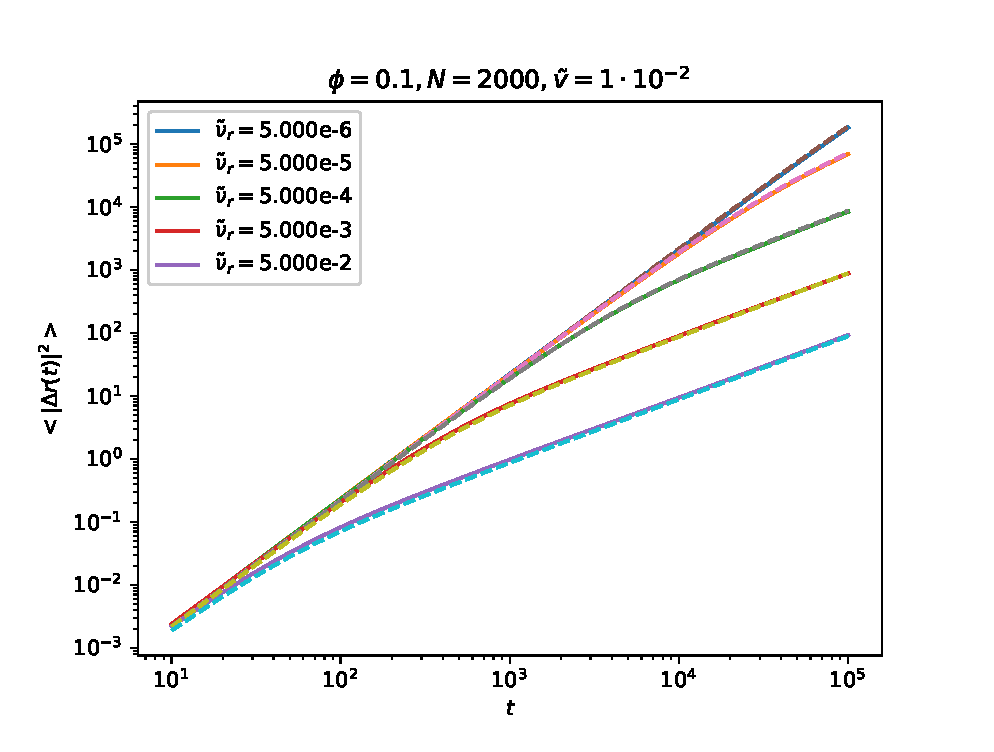
\includegraphics[width=0.6\textwidth]{figures/figs/msd_Dk1000_Vj1000_No2000.eps}
\caption{Mean square displacement as a function of time $\left<|\Delta\vec{r}(t)|^2\right>$, according to equation \ref{msd_ensemble}, for a system of $N=2\cdot10^3$ particles, with packing fraction $\phi=0.1$ and self-propulsion velocity $\tilde{v}=1\cdot10^{-2}$, for different rotational diffusion rates $\tilde{\nu}_r$. \textbf{(solid lines)} Computed mean square displacement at different rotational diffusion rates $\tilde{\nu}_r$. \textbf{(dashed lines)} Theoretical mean square displacement.}
\label{msd_ensemble_fit}
\end{figure}

\subsection{Equation of motion and control parameters}

From equations \ref{brownian_dynamics}, \ref{interparticle_force} and \ref{self_propulsion}, we can now write the equation of motion of particle $i$
\begin{equation}
\begin{aligned}
\frac{d}{dt}\vec{r}_i(t) &= \mu\left(\vec{F}_i^{(sp)}(t) + \sum_{j \neq i} \vec{F}_{ij}(t)\right)\\
&= \underbrace{v_0\vec{n}_i(t)\vphantom{\sum_{\substack{j \neq i \\ ||\vec{r}_i(t) - \vec{r}_j(t)|| < a_i + a_j}}}}_{\mathclap{\displaystyle\text{self-propulsion}}} + \underbrace{\mu \sum_{\substack{j \neq i \\ ||\vec{r}_i(t) - \vec{r}_j(t)|| < a_i + a_j}} k (a_i + a_j - ||\vec{r}_i(t) - \vec{r}_j(t)||)\frac{\vec{r}_i(t) - \vec{r}_j(t)}{||\vec{r}_i(t) - \vec{r}_j(t)||}}_{\displaystyle\text{interparticle interaction}}
\end{aligned}
\label{equation_motion}
\end{equation}
which we implement in our simulations.\\

We finally highlight the 3 control parameters of our model system \cite{fily2014freezing}:
\begin{itemize}
\item the packing fraction $\phi$,
\item the dimensionless self-propulsion velocity $\tilde{v} = v_0/ak$,
\item and the dimensionless rotational diffusion rate $\tilde{\nu}_r = \nu_r/k$ or equivalently the persistence time $\tau_r = \tilde{\nu}_r^{-1}$,
\end{itemize}
to which we will refer throughout this report.\\

An additional useful quantity is the dimensionless P\'eclet number, $\text{Pe} = \tilde{v}/\tilde{\nu}_r = \tilde{v}\tau_r$, which quantifies the dimensionless distance travelled by a single particle before its self-propulsion orientation decorrelates.

\section{Integration method}

Simulations were perfomed with the HOOMD-blue molecular dynamics simulation toolkit \cite{hoomd, anderson2008general, glaser2015strong, phillips2011pseudo} on Python \faPython. This toolkit was chosen for its high perfomance on GPUs, its versatility, and its ease of use. Our simulation script is available at \href{https://github.com/yketa/active_particles/blob/master/simulation/collective_migration_DPD_polydisperse_active.py}{{\faGithub~ yketa/active\_particles/simulation/collective\_migration\_DPD\_polydisperse\_active.py}}.

\myparagraph{Initialisation}

After setting the mean radius of particles $a = 1$, we choose the number $n_s$ of different radii of particles to be taken uniformly in the interval $[0.8; 1.2]$. As the algorithm runs slower with increasing $n_s$, we set $n_s = 10$ and then attribute to each particle one of these different radii. We choose the packing fraction $\phi$ and then set the length $L$ of the system square box accordingly.\\

We start by positioning particles randomly in the system box. We then use the Fast Inertial Relaxation Engine (FIRE) algorithm \cite{bitzek2006structural} to decrease particles' interpenetrations.

\myparagraph{Integration}

We set periodic boundary conditions and make use of the Brownian integrator as well as the active force functionality of HOOMD-blue for integration of equation \ref{equation_motion}.

\end{document}
